\chapter{Monte Carlo Solution Methods for Linear Systems}
\label{ch:stochastic_methods}
An alternative approach to approximate matrix inversion is to employ
Monte Carlo methods that sample a distribution with an expectation
value equivalent to that of the inverted operator. Such methods have
been in existence for decades with the earliest reference noted here
an enjoyable manuscript published in 1950 by Forsythe and Leibler
\citep{forsythe_matrix_1950}. In their outline, Forsythe and Liebler
in fact credit the creation of this technique to J. Von Neumann and
S.M. Ulam some years earlier than its publication. In 1952 Wasow
provided a more formal explanation of Von Neumann and Ulam's method
\citep{wasow_note_1952} and Hammersley and Handscomb's 1964 monograph
\citep{hammersley_monte_1964} and Spanier and Gelbard's 1969 book
\citep{spanier_monte_1969} present additional detail on this topic
using a collection of references from the 1950's and early 1960's.

\section{Preliminaries}
\label{sec:mc_preliminaries}
We begin our discussion of Monte Carlo methods using these texts by
seeking a solution to Eq~(\ref{eq:linear_problem}). For a given linear
operator $\ve{A}$, we can use diagonal splitting in a similar manner
as the stationary method in Eq~(\ref{eq:linear_split_equation2}) to
define the following operator\footnote{It should be noted that
  non-diagonal splittings have been recently explored in
  \citep{srinivasan_monte_2010} and have the potential to improve
  efficiency.}:
\begin{equation}
  \ve{H} = \ve{I} - \ve{A}\:,
  \label{eq:linear_mc_iteration_matrix}
\end{equation}
such that we are solving the system:
\begin{equation}
  \ve{x} = \ve{H} \ve{x} + \ve{b}\:.
  \label{eq:richardson_split}
\end{equation}
We can then form an alternative representation for $\ve{A}^{-1}$ by
generating the \textit{Neumann series}:
\begin{equation}
  \ve{A}^{-1} = (\ve{I}-\ve{H})^{-1} = \sum_{k=0}^{\infty} \ve{H}^k\:,
  \label{eq:neumann_series}
\end{equation}
which will converge if the spectral radius of $\ve{H}$ is less than
1. If we then apply this Neumann series to the right hand side of
Eq~(\ref{eq:linear_problem}) we acquire the solution to the linear
problem:
\begin{equation}
  \ve{A}^{-1}\ve{b} = \sum_{k=0}^{\infty} \ve{H}^k\ve{b} = \ve{x}\:.
  \label{eq:neumann_solution}
\end{equation}
An approximation of this summation by truncation will therefore lead
to an approximation of the solution. If we expand the summation with a
succession of matrix-vector multiply operations, we arrive at an
alternative perspective of this summation by considering its $i^{th}$
component:
\begin{equation}
  x_i = \sum_{k=0}^{\infty}\sum_{i_1}^{N}\sum_{i_2}^{N}\ldots
  \sum_{i_k}^{N}h_{i,i_1}h_{i_1,i_2}\ldots h_{i_{k-1},i_k}b_{i_k}\:,
  \label{eq:expanded_neumann_solution}
\end{equation}
which can interpreted as a series of transitions between states,
\begin{equation}
 \nu = i \rightarrow i_1 \rightarrow \cdots \rightarrow i_{k-1}
 \rightarrow i_{k}\:,
  \label{eq:mc_walk_permutation}
\end{equation}
in $\ve{H}$ where $\nu$ is interpreted as a particular random walk
sequence permutation. We can generate these sequences of transitions
through Monte Carlo random walks by assigning them both a probability
and weight. As a reinterpretation of the iteration matrix, we then
form the \textit{Neumann-Ulam decomposition} of \ve{H}:
\begin{equation}
  \ve{H} = \ve{P} \circ \ve{W}\:,
  \label{eq:neumann_ulam_decomposition}
\end{equation}
where $\circ$ denotes the Hadamard product operation\footnote{The
  Hadamard product $\ve{A} = \ve{B} \circ \ve{C}$ is defined
  element-wise as $a_{ij} = b_{ij} c_{ij}$.}, $\ve{P}$ denotes the
transition probability matrix, and $\ve{W}$ denotes the transition
weight matrix. This decomposition, a generalization of Dimov's work
\citep{dimov_new_1998}, is an extension of the original Neumann-Ulam
scheme in that now a weight cutoff can be used to terminate a random
walk sequence and therefore truncate the Neumann series it is
approximating. The formulation of $\ve{P}$ and $\ve{W}$ will be
dependent on whether we choose a direct or adjoint Monte Carlo
sequence to estimate the state transitions in
Eq~(\ref{eq:expanded_neumann_solution}).

\section{Direct Method}
\label{sec:direct_mc}
In the context of matrix inversion, a direct method resembles an
adjoint Monte Carlo method in the reactor physics community where the
solution state is sampled and the source terms that contribute to it
are assembled. To achieve this, we build the direct method
Neumann-Ulam decomposition per Dimov's approach by first choosing a
probability matrix that is a row scaling of $\ve{H}$ such that its
components are:
\begin{equation}
  p_{ij} = \frac{|h_{ij}|}{\sum_j |h_{ij}|}\:.
  \label{eq:direct_probability}
\end{equation}
From this, we then see that the probability of transitioning from a
state $i$ to a state $j$ is implicitly linked to the original operator
$\ve{A}$ in that those terms with large values, and therefore those
that make the greatest contribution to the numerical solution, will be
sampled with a higher probability than smaller terms. In addition, the
row scaling provides a normalization over the state to which we are
transitioning such that $\sum_j p_{ij} = 1$, meaning that we sample
the probabilities over the rows of the matrix. The components of
the weight matrix are then defined by
Eq~(\ref{eq:neumann_ulam_decomposition}) as:
\begin{equation}
  w_{ij} = \frac{h_{ij}}{p_{ij}}\:.
  \label{eq:direct_weight}
\end{equation}
It should be noted here that if $\ve{A}$ is sparse, then $\ve{H}$,
$\ve{P}$, and $\ve{W}$ must be sparse as well by
definition. Additionally, we only compute $\ve{P}$ and $\ve{W}$ from
the non-zero elements of $\ve{H}$ as those components that are zero
will not participate in the random walk. Doing so prevents an
infinite weight from being generated in Eq~(\ref{eq:direct_weight})
and eliminates unnecessary computations.

Using these matrices, we can then form the expectation value of the
direct solution. For a given random walk permutation $\nu$ with $k$
events, we define the weight of that permutation to be:
\begin{equation}
  W_{m} = w_{i,i_1} w_{i_1,i_2} \cdots w_{i_{m-1},i_m}\:,
  \label{eq:direct_permutation_weight}
\end{equation}
such that the weight of each transition event contributes to the
total. The contribution to the solution from a particular random walk
permutation is then:
\begin{equation}
  X_{\nu}(i_0 = i) = \sum_{m=0}^k W_{m} b_{i_m}\:,
  \label{eq:direct_permutation_contribution}
\end{equation}
where $X_{\nu}(i_0 = i)$ signifies that the solution state in which we
are tallying defines state $i$.  We can interpret this precisely as
before in that during the random walk we collect the source in the
states that are visited and apply them to the solution tally. We then
define the probability that a particular random walk permutation of
$k$ events will occur:
\begin{equation}
  P_{\nu} = p_{i,i_1} p_{i_1,i_2} \cdots p_{i_{k-1},i_k}\:.
  \label{eq:direct_permutation_probability}
\end{equation}
Finally, we define the expectation value of $X$ to be the collection
of all random walk permutations and their probabilities:
\begin{equation}
  E\{X(i_0 = i)\} = \sum_{\nu} P_{\nu} X_{\nu}\:,
  \label{eq:direct_expectation_value}
\end{equation}
which, if expanded, directly recovers the exact solution:
\begin{equation}
  \begin{split}
    E\{X(i_0 = i)\}
    &=\sum_{k=0}^{\infty}\sum_{i_1}^{N}\sum_{i_2}^{N}\ldots
    \sum_{i_k}^{N} p_{i,i_1}p_{i_1,i_2}\ldots p_{i_{k-1},i_k}
    w_{i,i_1}w_{i_1,i_2}\ldots w_{i_{k-1},i_k} b_{i_k}\\ &= x_i\:,
  \end{split}
  \label{eq:direct_expectation_expansion}
\end{equation}
therefore providing an unbiased Monte Carlo estimator. 

In cases where we seek only approximate solutions, we need only to
perform a minimal number of random walks in order to generate an
approximation for $\ve{x}$. If we are only to approximate the
solution, we also need conditions by which we may terminate a random
walk. We do this by noticing that the factors added to
Eq~(\ref{eq:direct_permutation_weight}) will become diminishingly
small due to their definition in Eq~(\ref{eq:direct_weight}) and
therefore their contributions to the solution estimate will become
negligible. Using this, we choose terminate a random walk sequence
with a \textit{weight cutoff}, $W_c$, that is enforced when $W_m <
W_c$ for a particular random walk permutation.

\subsection{Estimator Variance}
\label{subsec:estimator_variance}
We can compute the variance of the estimator through traditional
methods by defining the variance, $\sigma_i$, for each component in
the solution:
\begin{equation}
  {\sigma_i}^2 = E\{X(i_0 = i) - (\ve{A}^{-1}\ve{b})_i\}^2 = E\{X(i_0
  = i)^2\} - x_i^2\:,
  \label{eq:direct_variance_1}
\end{equation}
where the vector exponentials are computed element-wise. Inserting
Eq~(\ref{eq:direct_expectation_value}) gives:
\begin{equation}
  \sigma_i^2 = \Big(\sum_{\nu} P_{\nu} X_{\nu}^2\Big)_i - x_i^2\:,
  \label{eq:direct_variance_2}
\end{equation}
and applying Eq~(\ref{eq:direct_permutation_contribution}):
\begin{equation}
  \sigma_i^2 = \Big(\sum_{\nu} P_{\nu} \sum_{m=0}^k W_{m}^2
  b_{i_m}^2\Big)_i - x_i^2\:.
  \label{eq:direct_variance_3}
\end{equation}
Finally, expanding the transition probabilities yields the variance:
\begin{equation}
  \sigma_i^2 = \sum_{k=0}^{\infty}\sum_{i_1}^{N}\sum_{i_2}^{N}\ldots
  \sum_{i_k}^{N} p_{i,i_1}p_{i_1,i_2}\ldots p_{i_{k-1},i_k}
  w^2_{i,i_1}w^2_{i_1,i_2}\ldots w^2_{i_{k-1},i_k} b_{i_m} - x_i^2\:.
  \label{eq:direct_variance_4}
\end{equation}
Using this definition for the variance, we can arrive at a more natural
reason for enforcing $\rho(\ve{H}) < 1$ for our Monte Carlo method to
converge. Per the Hadamard product, we can concatenate the summation
in Eq~(\ref{eq:direct_variance_4}):
\begin{equation}
  (\ve{P} \circ \ve{W} \circ \ve{W})^k =
  \sum_{k=0}^{\infty}\sum_{i_1}^{N}\sum_{i_2}^{N}\ldots \sum_{i_k}^{N}
  p_{i,i_1}p_{i_1,i_2}\ldots p_{i_{k-1},i_k}
  w^2_{i,i_1}w^2_{i_1,i_2}\ldots w^2_{i_{k-1},i_k}\:.
  \label{eq:double_weighted_decomposition}
\end{equation}
If we assign $\ve{G} = \ve{P} \circ \ve{W} \circ \ve{W}$ as in
Eq~(\ref{eq:neumann_ulam_decomposition}), we then have a new
formulation for the variance:
\begin{equation}
  \sigma^2_i = \sum_{k=0}^{\infty}\sum_{i_1}^{N}\sum_{i_2}^{N}\ldots
  \sum_{i_k}^{N}g_{i,i_1}g_{i_1,i_2}\ldots g_{i_{k-1},i_k} b_{i_k}^2 -
  x_i^2\:,
\end{equation}
which contains the general Neumann series for $\ve{G}$,
\begin{equation}
  \ve{T} = \sum_{k=0}^{\infty} \ve{G}^k\:,
  \label{eq:variance_neumann_series}
\end{equation}
where $\ve{T} = (\ve{I}-\ve{G})^{-1}$. We can then insert $T$ back
into the variance formulation for a more concise definition:
\begin{equation}
  \sigma^2_i = (\ve{T}\ve{b})_i - x_i^2\:.
  \label{eq:direct_variance_5}
\end{equation}
We can relate $\ve{G}$ to $\ve{H}$ by noting that $\ve{G}$ simply
contains an additional Hadamard product with the weight matrix. The
Hadamard product has the property that:
\begin{equation}
  |\ve{H} \circ \ve{W}| \geq |\ve{H}|\ |\ve{W}|\:.
  \label{eq:hadamard_inequality}
\end{equation}
Using the norm property of the Hadamard product and
Eq~(\ref{eq:neumann_ulam_decomposition}), we can define the norm of
$\ve{W}$ as:
\begin{equation}
  \frac{|\ve{H}|}{|\ve{P}|} \geq |\ve{W}|\:.
  \label{eq:weight_norm}
\end{equation}
Choosing the infinity norm of the operator as defined in
Eq~(\ref{eq:matrix_infinity_norm}), the row normalized probability
matrix will yield a norm of 1 giving the following inequality for
relating $\ve{G}$ and $\ve{H}$:
\begin{equation}
  |\ve{G}| \geq |\ve{H}|^2
  \label{eq:variance_norm_inequality}
\end{equation}
Using these relations to analyze Eq~(\ref{eq:direct_variance_5}), we
see that if $\rho(\ve{G}) > 1$, then the sum in
Eq~(\ref{eq:variance_neumann_series}) will not converge and an
infinite variance will arise as the elements of $\ve{T}$ become
infinite in Eq~(\ref{eq:direct_variance_5}). We must restrict $\ve{G}$
to alleviate this and therefore restrict $\ve{H}$ due to
Eq~(\ref{eq:variance_norm_inequality}) with $\rho(\ve{H}) < 1$ so that
our expectation values for the solution may have a finite variance.

\subsection{Reusing Random Walks}
\label{subsec:reusing_random_walks}
A downfall of the direct method is that a random walk must be
initiated in each state of the solution vector in which the solution
is desired due to the estimator definition in
Eq~(\ref{eq:direct_expectation_expansion}). Because of this, a
solution estimate in all states of a linear system may require a
large number of random walks to be performed. Ji and Li recently
proposed a variation of the direct method in which the random walk
permutations in Eq~(\ref{eq:mc_walk_permutation}) can be used to
contribute to the solution tally in all visited states instead of the
only starting state \citep{ji_reusing_2012}. By doing this, they
effectively reduce the number of random walks needed to sample all
desired states in the system.

Their method is based on the observation that while a random walk
transitions between states in the system, if every state it visited
could be considered that starting state, then a series a contributions
to the solution could be generated by a single sequence of random
numbers while maintaining statistical independence between the
samples. To demonstrate this, consider the following random walk
sequence starting in state 2: $2 \rightarrow 3 \rightarrow 1
\rightarrow 2 \rightarrow 4 \rightarrow 5$. We can reuse these walks
be recognizing that we also then have a random walk sequence starting
in state 3 that can be applied to the state 3 estimator: $3
\rightarrow 1 \rightarrow 2 \rightarrow 4 \rightarrow 5$. We also have
the same situation for state 1: $1 \rightarrow 2 \rightarrow 4
\rightarrow 5$, and all future states. Using this sampling scheme , Ji
and Li observed 1 to 2 orders of magnitude reduction over the standard
direct method in the number histories required to achieve a specified
variance in their test problems.

\section{Adjoint Method}
\label{sec:adjoint_mc}
An alternative formulation for Monte Carlo matrix inversion is the
adjoint method. We begin by defining the linear system adjoint to
Eq~(\ref{eq:linear_problem}):
\begin{equation}
  \ve{A}^T \ve{y} = \ve{d}\:,
  \label{eq:adjoint_linear_problem}
\end{equation}
where $\ve{y}$ and $\ve{d}$ are the adjoint solution and source
respectively and $\ve{A}^T$ is the adjoint operator. We can split this
equation to mirror Eq~(\ref{eq:richardson_split}) by defining the
following inner product equivalence \citep{spanier_monte_1969}:
\begin{equation}
  \langle \ve{A}^T \ve{x}, \ve{y} \rangle = \langle \ve{x}, \ve{A}
  \ve{y} \rangle\:.
  \label{eq:adjoint_operator_product}
\end{equation}
With this statement we can then define the split equation:
\begin{equation}
  \ve{y} = \ve{H}^T \ve{y} + \ve{d}\:.
  \label{eq:adjoint_split_system}
\end{equation}
As was required for convergence with the direct method using
Eq~(\ref{eq:richardson_split}), the spectral radius of $\ve{H}$ must
remain less than 1 as $\ve{H}^T$ contains the same eigenvalues and
therefore has the same spectral radius. From this definition it
follows that:
\begin{equation}
  \langle \ve{x}, \ve{d} \rangle = \langle \ve{y}, \ve{b} \rangle\:.
  \label{eq:adjoint_vector_relation}
\end{equation}
Using these definitions, we can derive an estimator from the adjoint
method that will also give the solution vector, $\ve{x}$. As with the
direct method, we can acquire the adjoint solution by forming the
Neumann series by writing Eq~(\ref{eq:adjoint_split_system}) as:
\begin{equation}
  \ve{y} = (\ve{I} - \ve{H}^T)^{-1} \ve{d}\:,
  \label{eq:adjoint_split_system_2}
\end{equation}
which in turn yields the Neumann series using the adjoint operator:
\begin{equation}
  \ve{y} = \sum_{k=0}^{\infty} (\ve{H}^T)^k\ve{d}\:.
  \label{eq:adjoint_neumann_series}
\end{equation}
We expand this summation to again yield a series of transitions that
can be approximated by a Monte Carlo random walk sequence, this time
forming the Neumann series in reverse order:
\begin{equation}
  y_i = \sum_{k=0}^{\infty}\sum_{i_1}^{N}\sum_{i_2}^{N}\ldots
  \sum_{i_k}^{N}h_{i_k,i_{k-1}}\ldots h_{i_2,i_1} h_{i_1,i} d_{i_k}\:.
  \label{eq:adjoint_neumann_solution}
\end{equation}
We can readily build an estimator for the adjoint solution from this
series expansion, but we instead desire the direct solution. We
achieve this by using Eq~(\ref{eq:adjoint_vector_relation}) as a
constraint. Here we have 2 unknowns, $\ve{y}$ and $\ve{d}$ and
therefore we require a second constraint to close the system. As a
second constraint we select:
\begin{equation}
  \ve{d} = \boldsymbol{\delta}_i\:,
  \label{eq:adjoint_second_constraint}
\end{equation}
where the $k^{th}$ component of the vector $\boldsymbol{\delta}_i$ is
the Dirac delta function $\delta_{i_k,i}$. If we apply
Eq~(\ref{eq:adjoint_second_constraint}) to our first constraint
Eq~(\ref{eq:adjoint_vector_relation}), we get the following convenient
outcome:
\begin{equation}
  \langle \ve{y}, \ve{b} \rangle = \langle \ve{x},
  \boldsymbol{\delta}_i \rangle = x_i \:,
  \label{eq:inner_product_constraint}
\end{equation}
meaning that if we compute the inner product of the direct source and
the adjoint solution using a delta function source, we recover the
direct solution we are looking for 

In terms of particle transport, this adjoint method is equivalent to a
traditional forward method. As a result of using the adjoint system,
we modify our probabilities and weights using the \textit{adjoint
  Neumann-Ulam decomposition} of $\ve{H}$:
\begin{equation}
  \ve{H}^{T} = \ve{P} \circ \ve{W}\:,
  \label{eq:adjoint_neumann_ulam}
\end{equation}
where now we are forming the decomposition with respect to the
transpose of $\ve{H}$\footnote{This is sometimes referred to as the
  adjoint form for real-valued matrices}. We then follow the same
procedure as the direct method for forming the probability and weight
matrices in the decomposition. Using the adjoint form, probabilities
should instead be column-scaled:
\begin{equation}
  p_{ij} = \frac{|h_{ji}|}{\sum_j |h_{ji}|}\:,
  \label{eq:adjoint_probability}
\end{equation}
such that we expect to select a new state $j$ from the current state
in the random walk $j$ by sampling column-wise. Per
Eq~(\ref{eq:adjoint_neumann_ulam}), the transition weight is then
defined as:
\begin{equation}
  w_{ij} = \frac{h_{ji}}{p_{ij}}\:.
  \label{eq:adjoint_weight}
\end{equation}
Using the decomposition we can then define an expectation value for
the adjoint method. Given Eq~(\ref{eq:direct_permutation_weight}) as
the weight generated for a particular random walk permutation as in
Eq~(\ref{eq:mc_walk_permutation}) and our result from
Eq~(\ref{eq:inner_product_constraint}) generated by applying the
adjoint constraints, the contribution to the solution in state $i$
from a particular random walk permutation is then:
\begin{equation}
  X_{\nu} = \sum_{m=0}^k W_{m} \delta_{i,i_m}\:,
  \label{eq:adjoint_permutation_contribution}
\end{equation}
where the Kronecker delta indicates that the tally contributes only in
the current state and $b_{i_0}$ will be the sampled source starting
weight. Note here that the estimator in
Eq~(\ref{eq:adjoint_permutation_contribution}) does not have a
dependency on the source state as in
Eq~(\ref{eq:adjoint_permutation_contribution}), providing a remedy for
the situation in the direct method where we must start a random walk
in each source state for every permutation such that we may compute a
contribution for that state. In the adjoint method, we instead tally
in all states and those of lesser importance will not be visited as
frequently by the random walk. Finally, the expectation value using
all permutations is:
\begin{equation}
  E\{X\} = \sum_{\nu} P_{\nu} X_{\nu}\:
  \label{eq:adjoint_expectation_value}
\end{equation}
which, if expanded in the same way as the direct method, directly
recovers the exact solution:
\begin{equation}
  \begin{split}
    E\{X_j\} &=\sum_{k=0}^{\infty}\sum_{i_1}^{N}\sum_{i_2}^{N}\ldots
    \sum_{i_k}^{N} b_{i_0} h_{i_0,i_1}h_{i_1,i_2}\ldots h_{i_{k-1},i_k}
    \delta_{i_k,j} \\ &= x_{j}\:,
  \end{split}
  \label{eq:adjoint_expectation_expansion}
\end{equation}
therefore also providing an unbiased Monte Carlo estimate of the
solution.

Like the direct method, we also desire a criteria for random walk
termination for problems where only an approximate solution is
necessary. For the adjoint method, we utilize a \textit{relative
  weight cutoff}:
\begin{equation}
  W_f = W_c b_{i_0}\:,
  \label{eq:relative_weight_cutoff}
\end{equation}
where $W_c$ is defined as in the direct method. The adjoint random
walk will then be terminated after $m$ steps if $W_m < W_f$ as tally
contributions become increasingly small.

\section{Sequential Monte Carlo}
\label{sec:sequential_mc}
The direct and adjoint Neumann-Ulam methods described are limited by a
convergence rate of $1/\sqrt{N}$ by the Central Limit Theorem where
$N$ is the number of random walk permutations. In 1962, Halton
presented a residual Monte Carlo method that moves towards exponential
convergence rates \citep{halton_sequential_1962} and further refined
his work some years later \citep{halton_sequential_1994}. Applications
of his work by the transport community have confirmed convergence
rates on the order of of $exp(-N)$ \citep{evans_residual_2003}. In
much the same way as projection methods, Halton's method, sequential
Monte Carlo, utilizes the adjoint Monte Carlo solver as a means of
directly reducing the residual vector. He proposed the following
iterative scheme as a solution to Eq~(\ref{eq:linear_problem})\:
\begin{subequations}
  \begin{gather}
    \ve{r}^k = \ve{b} - \ve{A}\ve{x}^k\:,\\  
    \ve{A}\boldsymbol{\delta}^{k} = \ve{r}^{k}\:,\\
    \ve{x}^{k+1} = \ve{x}^k + \boldsymbol{\delta}^{k}\:,
  \end{gather}
  \label{eq:sequential_monte_carlo}
\end{subequations}
where the correction $\boldsymbol{\delta}$ is computed by the adjoint
Monte Carlo method. The merits of Halton's approach are immediately
visible in that we have now broken the binding of the convergence rate
to the Central Limit Theorem. Here, the Monte Carlo solver is used to
produce a correction from the residual, analogous to using the
residual to extract a correction from the search subspace in a
projection method. By doing this, the Monte Carlo error is bound in
the correction used to update the solution and therefore does not
explicitly manifest itself in the overall convergence of the
solution. The downside of such a method is that if the solution guess
is poor, then many iterations are required in order to reach
exponential converge as the Monte Carlo error (and therefore the
Central Limit Theorem) does dominate in this situation. Therefore, if
a good initial guess is not available, Halton's method is still
characterized by poor performance.

\section{Monte Carlo Synthetic-Acceleration}
\label{sec:mcsa}
Using the ideas of Halton, Evans and Mosher recently developed a Monte
Carlo solution method that was not prohibited severely by the quality
of the initial guess for the system \citep{evans_monte_2009} and later
applied it more rigorously as a solution mechanism for the radiation
diffusion equation \citep{evans_monte_2012}. With their new methods,
they achieved identical numerical results as and marginally better
performance than conventional Krylov solvers. Their approach was
instead to use residual Monte Carlo as a synthetic acceleration for a
stationary method. To derive this method, we begin by splitting the
operator in Eq~(\ref{eq:linear_problem})
\begin{equation}
  \ve{x} = (\ve{I} - \ve{A})\ve{x} + \ve{b}\:.
  \label{eq:linear_split}
\end{equation}
With this we can then define the stationary method
\textit{Richardson's iteration} as:
\begin{equation}
  \ve{x}^{k+1} = (\ve{I} - \ve{A})\ve{x}^k + \ve{b}\:,
  \label{eq:richardsons_iteration}
\end{equation}
which will converge if $\rho(\ve{I} - \ve{A}) < 1$. We then define the
solution error at the $k^{th}$ iterate relative to the true solution:
\begin{equation}
  \delta \ve{x}^k = \ve{x} - \ve{x}^k\:.
  \label{eq:mcsa_error}
\end{equation}
Subtracting Eq~(\ref{eq:richardsons_iteration}) from
Eq~(\ref{eq:linear_split}) we get:
\begin{equation}
  \delta \ve{x}^{k+1} = (\ve{I} - \ve{A})\delta \ve{x}^k\:.
  \label{eq:mcsa_setup_1}
\end{equation}
Subtracting from this $(\ve{I} - \ve{A})\delta \ve{x}^{k+1}$ yields:
\begin{equation}
  \begin{split}
    \ve{A}\delta \ve{x}^{k+1} &= (\ve{I} -
    \ve{A})(\ve{x}^{k+1}-\ve{x}^{k}) \\ &= \ve{r}^{k+1}\:.
    \label{eq:mcsa_setup_2}
  \end{split}
\end{equation}
Using this, we define the following scheme that will converge in one
iteration if $\ve{A}$ is inverted exactly.
\begin{subequations}
  \begin{gather}
    \ve{x}^{k+1} = (\ve{I} - \ve{A})\ve{x}^k + \ve{b}\:,\\
    \ve{A} \delta \ve{x}^{k+1} = \ve{r}^{k+1}\:,\\
    \ve{x} = \ve{x}^{k+1} + \delta \ve{x}^{k+1}\:.
  \end{gather}
  \label{eq:mcsa_setup_3}
\end{subequations}
However, $\ve{A}$ is only approximately inverted by our numerical
methods and therefore we instead pose an iterative scheme in which the
Monte Carlo solvers are used to invert the operator. The
\textit{Fixed-Point Monte Carlo Synthetic-Acceleration} (MCSA) method
is defined as:
\begin{subequations}
  \begin{gather}
    \ve{x}^{k+1/2} = (\ve{I} - \ve{A})\ve{x}^k + \ve{b}\:,\\
    \ve{r}^{k+1/2} = \ve{b} - \ve{A}\ve{x}^{k+1/2}\:,\\
    \ve{A}\delta\ve{x}^{k+1/2} = \ve{r}^{k+1/2}\:,\\
    \ve{x}^{k+1} = \ve{x}^{k+1/2} + \delta \ve{x}^{k+1/2}\:,
  \end{gather}
  \label{eq:mcsa}
\end{subequations}
where the adjoint Monte Carlo method is used to generate the solution
correction from the residual. Using Monte Carlo in this way achieves
the same effect as Halton's method, decoupling its convergence rate
from the overall convergence rate of the method. Here, the approximate
Monte Carlo solution is not driven to a particular convergence as it
merely supplies a correction for the initial guess generated by
Richardson's iteration. Rather, only a set number of histories are
required using the adjoint method to generate the correction.

In addition to the Monte Carlo solver parameters dictating the number
of histories and weight cutoff, the outer MCSA iterations also have
the following stopping criteria:
\begin{equation}
  ||\ve{r}||_\infty < \epsilon \ ||\ve{b}||_\infty\:,
  \label{eq:mcsa_stopping_criteria}
\end{equation}
where $\epsilon$ is a user-defined parameter. We therefore have 3
parameters to tune in an MCSA implementation: the number of Monte
Carlo histories computed in the adjoint solve during each MCSA
iteration, the weight cutoff for those histories, and the total MCSA
convergence tolerance as specified by $\epsilon$.

\subsection{Preconditioning MCSA}
\label{sec:stochastic_preconditioning}
In most cases, at least a minimal amount of \textit{preconditioning}
of the linear system will be required in order to use the class of
stochastic methods described. Although these methods have no symmetry
requirements for convergence, they do require that the spectral radius
of the iteration matrix be less than one. To achieve this, a Jacobi
preconditioner, a form of left preconditioning, is used such that the
preconditioning matrix $\ve{M}$ is:
\begin{equation}
  \ve{M} = diag(\ve{A})\:,
  \label{eq:jacobi_preconditioner}
\end{equation}
such that its application means we are instead solving the following
linear system:
\begin{equation}
  \ve{M}^{-1}\ve{A}\ve{x} = \ve{M}^{-1}\ve{b}\:.
  \label{eq:jacobi_precond_linear_problem}
\end{equation}
Next, we can apply MCSA to solve
Eq~(\ref{eq:jacobi_precond_linear_problem}): 
\begin{subequations}
  \begin{gather}
    \ve{x}^{k+1/2} = (\ve{I} - \ve{M}^{-1}\ve{A})\ve{x}^k +
    \ve{M}^{-1}\ve{b}\:,\\ \ve{r}^{k+1/2} = \ve{M}^{-1}\ve{b} -
    \ve{M}^{-1}\ve{A}\ve{x}^{k+1/2}\:,\\ \ve{M}^{-1}\ve{A}\delta\ve{x}^{k+1/2}
    = \ve{r}^{k+1/2}\:,\\ \ve{x}^{k+1} = \ve{x}^{k+1/2} + \delta
    \ve{x}^{k+1/2}\:.
    \label{eq:jacobi_preconditioned_mcsa}
  \end{gather}
\end{subequations}
Choosing Jacobi preconditioning with MCSA is advantageous for several
reasons. First, $\rho(\ve{I} - \ve{M}^{-1}\ve{A}) < 1$ is true for all
$\ve{A}$ and is easy to formulate because the inversion of $\ve{M}$ is
trivial. Second, because the adjoint Monte Carlo method used within
MCSA to compute the correction operates on a linear problem with the
preconditioned operator, then $\ve{H}$ in the adjoint solver will have
a zero term in each of its diagonal elements, thereby eliminating all
in-state transitions during the random walk sequence. Because of this,
Jacobi preconditioning should always be performed, regardless of any
other preconditioning that is applied to the system.

\section{Monte Carlo Method Selection}

The MCSA method defined in Eq.~(\ref{eq:mcsa}) uses the adjoint method
to estimate the error in residual Monte Carlo solve instead of the
direct method outlined in \S~\ref{sec:direct_mc}. To demonstrate
the effectiveness of the adjoint method over the direct method within
the context of MCSA, we choose the 2D time-dependent Poisson equation
as a simple model problem:
\begin{equation}
  \frac{\partial \ve{u}}{\partial t} = \nabla^2 \ve{u}\:.
  \label{eq:poisson_equation}
\end{equation}
For all comparisons, a single time step is computed with backwards Euler time
integration. The Laplacian is differenced on a square Cartesian grid with a
second-order five-point stencil,
\begin{equation}
  \nabla^2_5 = \frac{1}{\Delta^2}[u_{i-1,j} + u_{i+1,j} + u_{i,j-1} +
    u_{i,j+1} - 4 u_{i,j}]\:,
  \label{eq:five_point_stencil}
\end{equation}
and a fourth-order nine-point stencil,
\begin{multline}
  \nabla^2_9 = \frac{1}{6\Delta^2}[4 u_{i-1,j} + 4 u_{i+1,j} + 4
    u_{i,j-1} + 4 u_{i,j+1} + u_{i-1,j-1}\\ + u_{i-1,j+1} +
    u_{i+1,j-1} + u_{i+1,j+1} - 20 u_{i,j}]\:,
  \label{eq:nine_point_stencil}
\end{multline}
both assuming a grid size of $\Delta$ in both the $i$ and $j$ directions. For
a single time step solution, we then have the following sparse linear system
to be solved with the MCSA method:
\begin{equation}
  \ve{A} \ve{u}^{n+1} = \ve{u}^n\:.
  \label{eq:poisson_eq_lin_sys}
\end{equation}
Both the stencils will be used to vary the size and density of the sparse
linear system in Eq.~(\ref{eq:poisson_eq_lin_sys}).

A timing and convergence study is used to demonstrate the
effectiveness of the adjoint method as compared to the direct
method. To assess both the CPU time and number of iterations required
to converge to a solution, a problem of constant $\Delta$ was used
with varying values of grid size, fixing the spectral radius of the
system at a constant value for each variation. Both the five-point and
nine-point stencils were used with both the direct and adjoint
solvers. For each case, $N \times N$ total random walk permutations
were computed per MCSA iteration where $N \times N$ is the number of
discrete grid points in the system. Solver parameters were set to a
weight cutoff of \sn{1}{-4} for the stochastic linear solver and a
convergence tolerance of \sn{1}{-8} for the MCSA iterative solver.
Figure~\ref{fig:poisson_cpu_time} gives the CPU time needed for each
case to converge in seconds and Figure~\ref{fig:poisson_iterations}
gives the number of iterations needed for each case to converge to the
specified tolerance as a function of the problem size. All
computations presented in this section and
\S~\ref{subsec:sequential_comparison} were completed on a 3.0 GHz
Intel Core 2 Quad Q9650 CPU machine with 16 GB 1067 MHz DDR3 memory.
\begin{figure}[ht!]
  \centering
  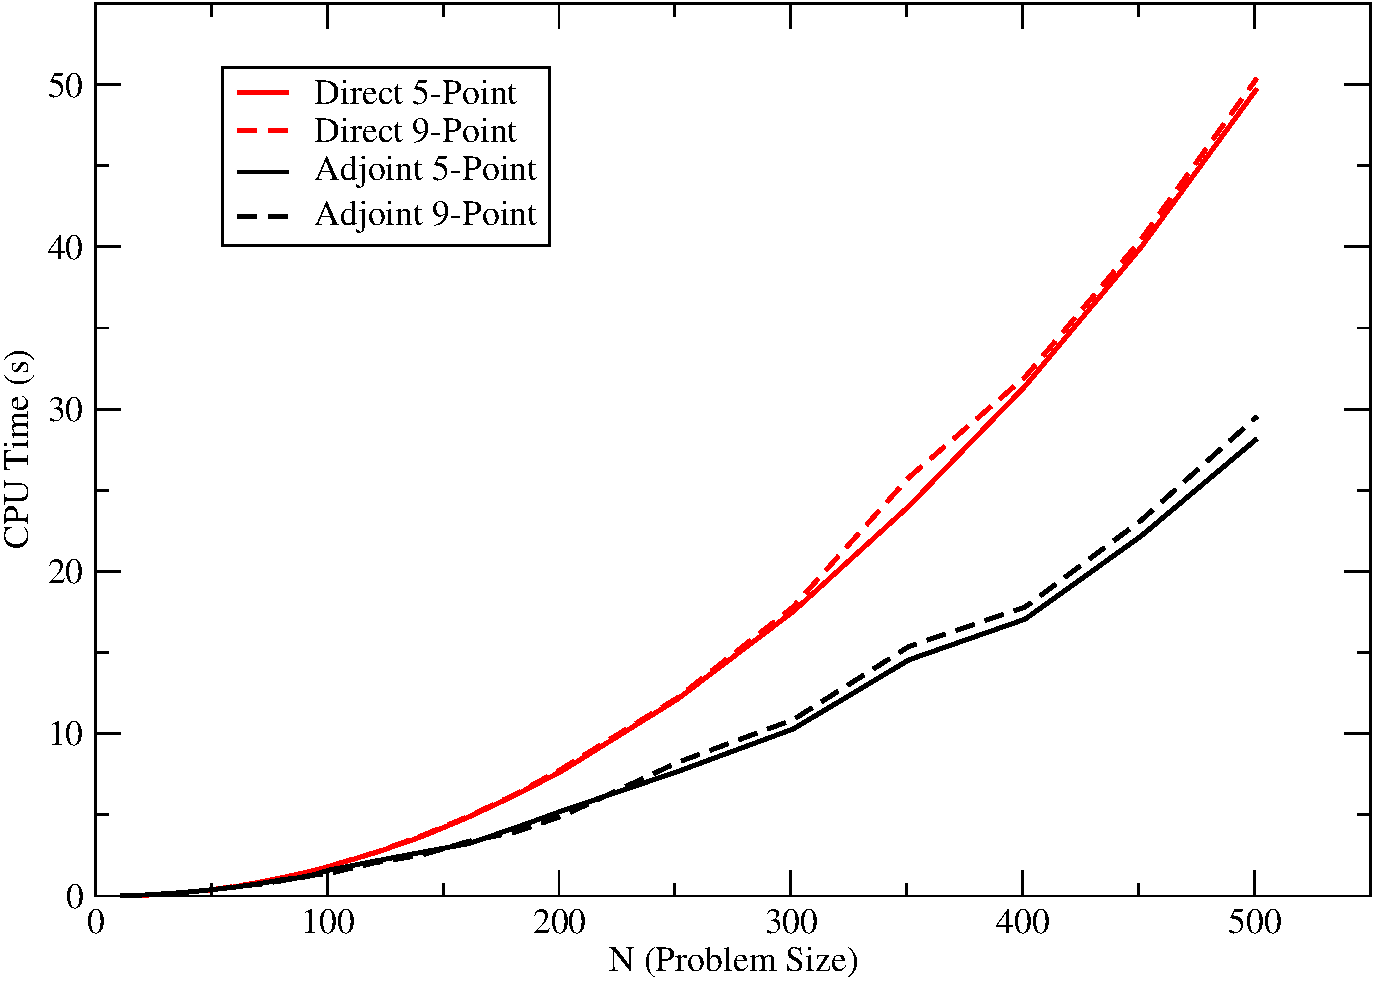
\includegraphics[width=5in,clip]{chapters/mc_background/dir_adj_cpu.pdf}
  \caption{\textbf{CPU Time (s) to converge vs. Problem Size ($N$ for
      an $N \times N$ square mesh).} \textit{Both the adjoint and
      direct solvers are used with the five point and nine point
      stencils. A CPU time speedup is noted with the adjoint method
      due to the higher density of random walk events in regions with
      a large residual.}}
  \label{fig:poisson_cpu_time}
\end{figure}

\begin{figure}[ht!]
  \centering
  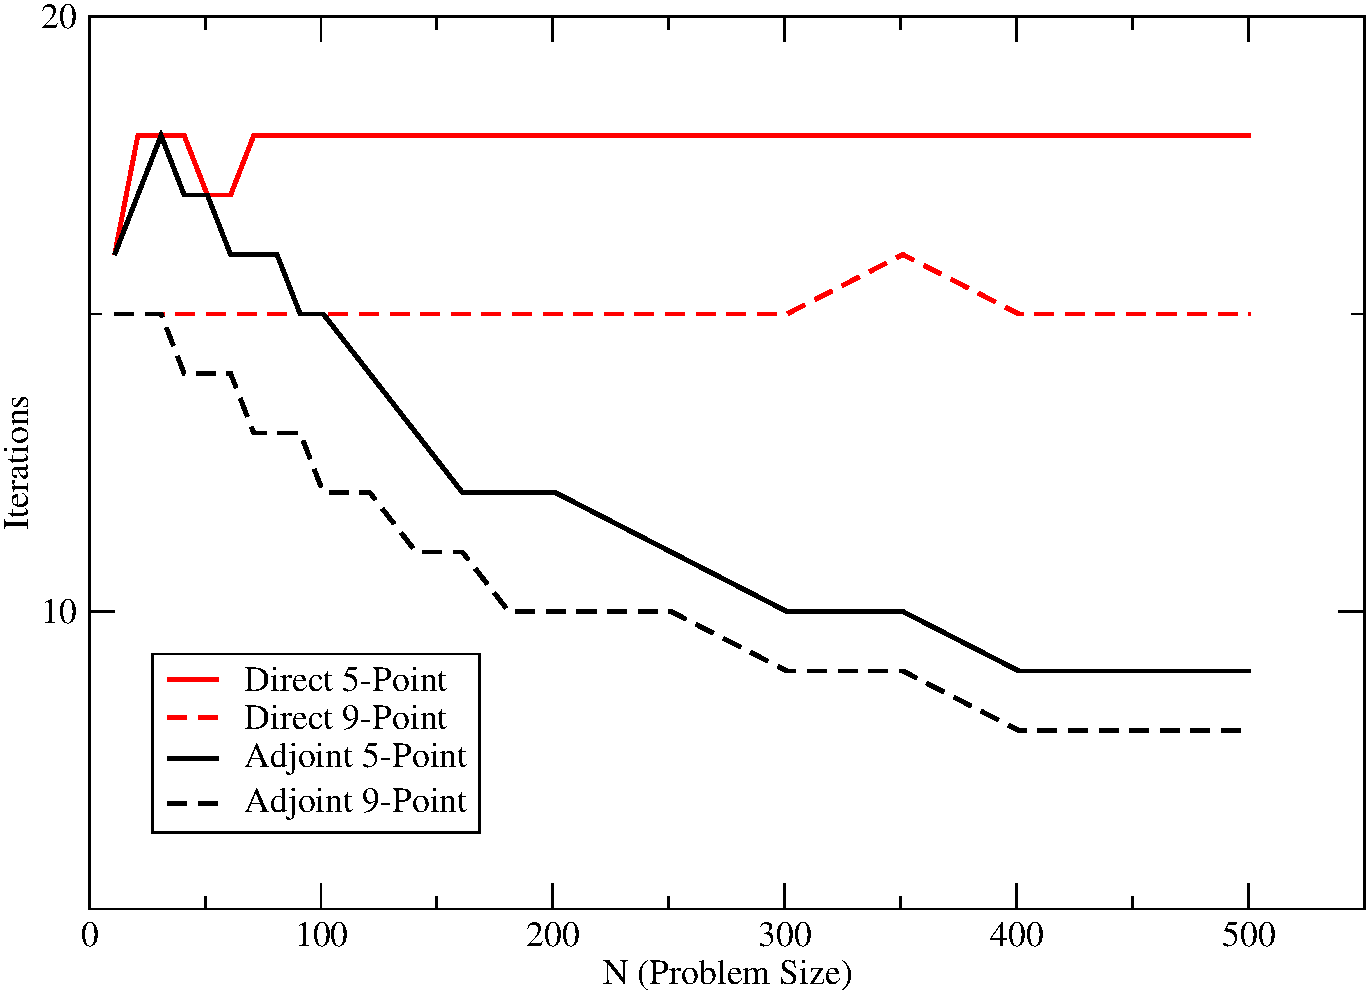
\includegraphics[width=5in,clip]{chapters/mc_background/dir_adj_iterations.pdf}
  \caption{\textbf{Iterations to converge vs. Problem Size ($N$ for an
      $N \times N$ square mesh).} \textit{Both the adjoint and direct
      solvers are used with the five-point and nine-point stencils.}}
  \label{fig:poisson_iterations}
\end{figure}

We see clearly in Figure~\ref{fig:poisson_cpu_time} that the using the
adjoint solver with MCSA results in a speedup over the direct solver
while the number of iterations required to converge is also reduced as
shown in Figure~\ref{fig:poisson_iterations}. We expect this for several
reasons. First, with an equivalent number of histories specified for
both solvers per MCSA iteration and a system of size $N \times N$, the
direct solver will compute a single random walk for each state in the
system per iteration to acquire a solution in that state, regardless
of the size of the residual in that state. This is necessary in the
direct method to ensure a contribution from each state as the random
walk sequence will only contribute to the starting state. For the
adjoint method, a total of $N \times N$ random walk events will have
their starting state determined by sampling the residual
vector. Because the random walk sequence contributes to the state in
which it currently resides, sampling the residual vector as the Monte
Carlo source gives a higher density of random walk events in regions
with a high residual, thus giving a more accurate correction in that
region due to reduced statistical error. From an iteration
perspective, Figure~\ref{fig:poisson_iterations} shows that using the
direct method yields a roughly unchanging number of iterations
required to converge as the problem size increases. Again, if we
desire a correction value for all states in the problem, then we must
start a random walk in each state in the system which does not reduce
the number of iterations need as the problem size grows. Conversely,
as the problem size grows in the adjoint method, the additional
stochastic histories that will be computed are concentrated in regions
with a large residual, further reducing the stochastic error in the
correction in those regions and subsequently reducing the required
number of iterations to converge.

As an additional comparison, the convergence behavior of MCSA can be
analyzed using both the adjoint and direct solvers to detect any
performance benefits. To assess the convergence properties of MCSA
using each solver and stencil, the infinity norm of the residual
computed in Eq.~(\ref{eq:mcsa}) was collected at each iteration for a
fixed problem size of $N=500$. Figure~\ref{fig:poisson_convergence}
gives the results of these computations. First, it is worthy to note
on the semilog plot that we are indeed achieving the expected
exponential convergence from MCSA with both Monte Carlo
solvers. Second, we note that using the adjoint method with the same
number of stochastic histores per MCSA iteration gives a faster rate
of converge for the same reasons as above. We also note here that
fewer iterations are required for convergence when the 9-point stencil
is used to discretize the Laplacian operator (although at no gain in
speed as given by the results in
Figure~\ref{fig:poisson_cpu_time}). This is due to the fact that the
smaller discretization error directly corresponds to a more well
defined residual source generated by the Richardson extrapolation for
the Monte Carlo calculation. In addition, the better defined source is
transported through a domain described more accurately by the 9-point
stencil, thus yielding a more accuracte correction vector from the
Monte Carlo calculation.
\begin{figure}[ht!]
  \centering
  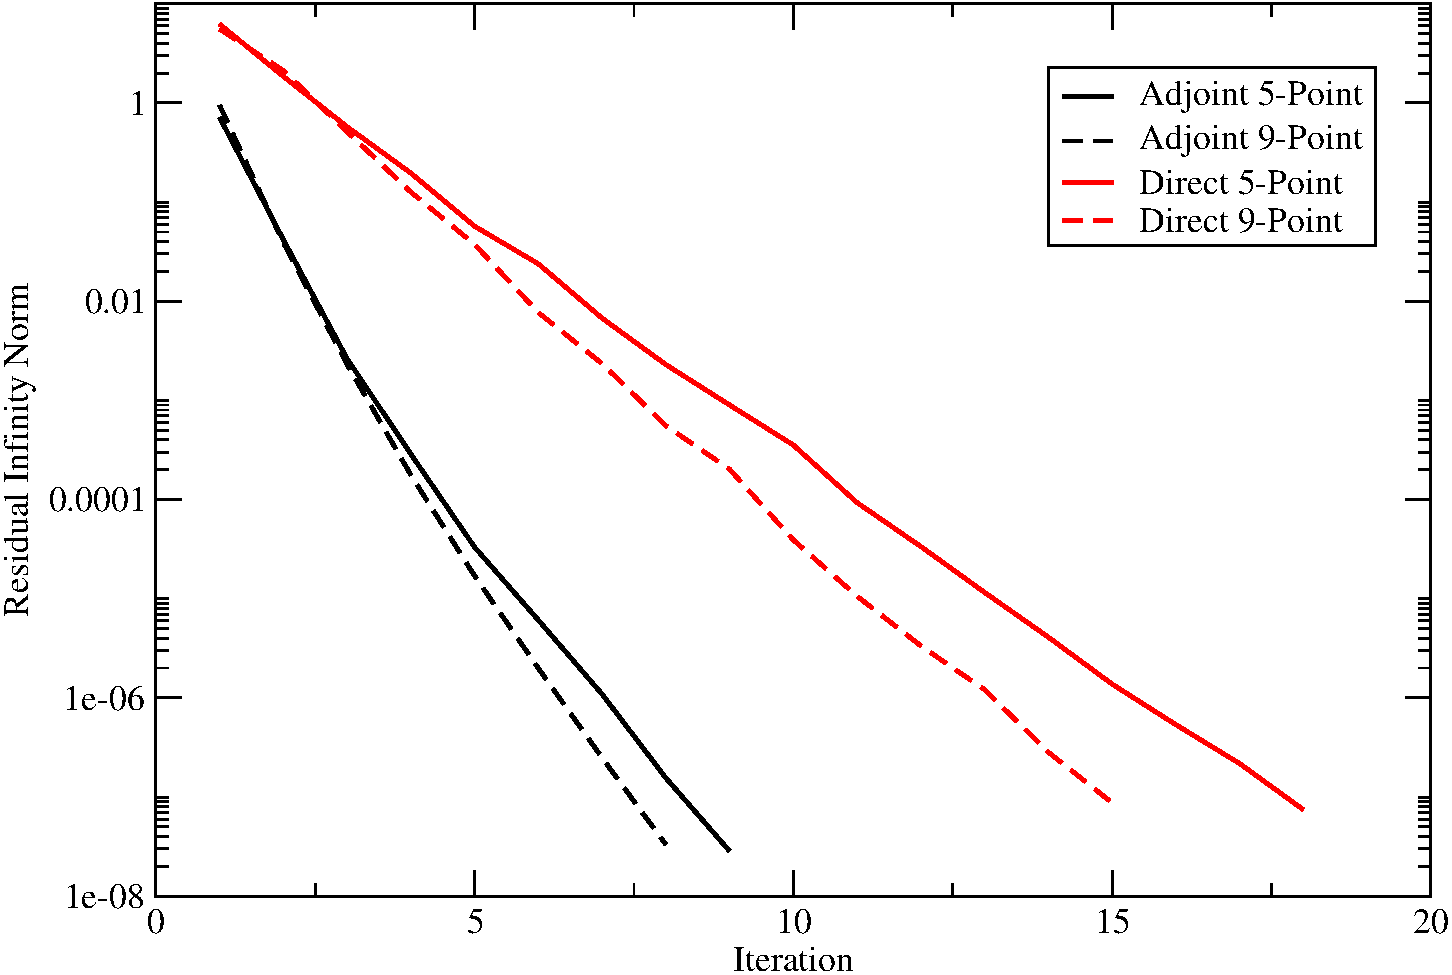
\includegraphics[width=5in,clip]{chapters/mc_background/dir_adj_conv.pdf}
  \caption{\textbf{Infinity norm of the solution residual
      vs. iteration number for a problem of size $N=500$.}
    \textit{Both the adjoint and direct solvers are used with the five
      point and nine point stencils. A higher rate of convergence is
      observed for MCSA using the adjoint Monte Carlo solver as
      compared to the direct method when both solvers compute the same
      number of random walks per iteration.}}
  \label{fig:poisson_convergence}
\end{figure}

\section{Comparison to Sequential Monte Carlo}
\label{subsec:sequential_comparison}
To further motivate using Monte Carlo Synthetic Acceleration, we
compare its performance to Halton's Sequential Monte Carlo method on
which our previous work in this area was based. For this comparison,
we use the same transient Poisson problem as described in the previous
section and choose only the 5-point stencil to discretize the
Laplacian operator as the previous results yielded little qualitative
difference between the discretizations. Both MCSA and Halton's method
are used with the adjoint Monte Carlo solver. In order to complete the
same study as in the previous section, the number of histories
computed by the Monte Carlo solver at each iteration had to be doubled
to $2 \times N \times N$ in order to ensure convergence in Sequential
Monte Carlo Method. Figure~\ref{fig:seq_cpu_time} gives the CPU time
results for this comparison as a function of problem size while
Figure~\ref{fig:seq_iterations} gives the number of iterations to
converge as a function of problem size. In both cases, using the Monte
Carlo solver as a synthetic acceleration rather than in a pure
residual Monte Carlo scheme resulted in a reduction in both CPU time
and iterations required to converge. The additional Richardson
extrapolation between each Monte Carlo solve in the MCSA method gives
a better converged residual source to use with the Monte Carlo
calculation while the Sequential method requires more iterations to
achieve the same level of convergence in the residual.

\begin{figure}[ht!]
  \centering
  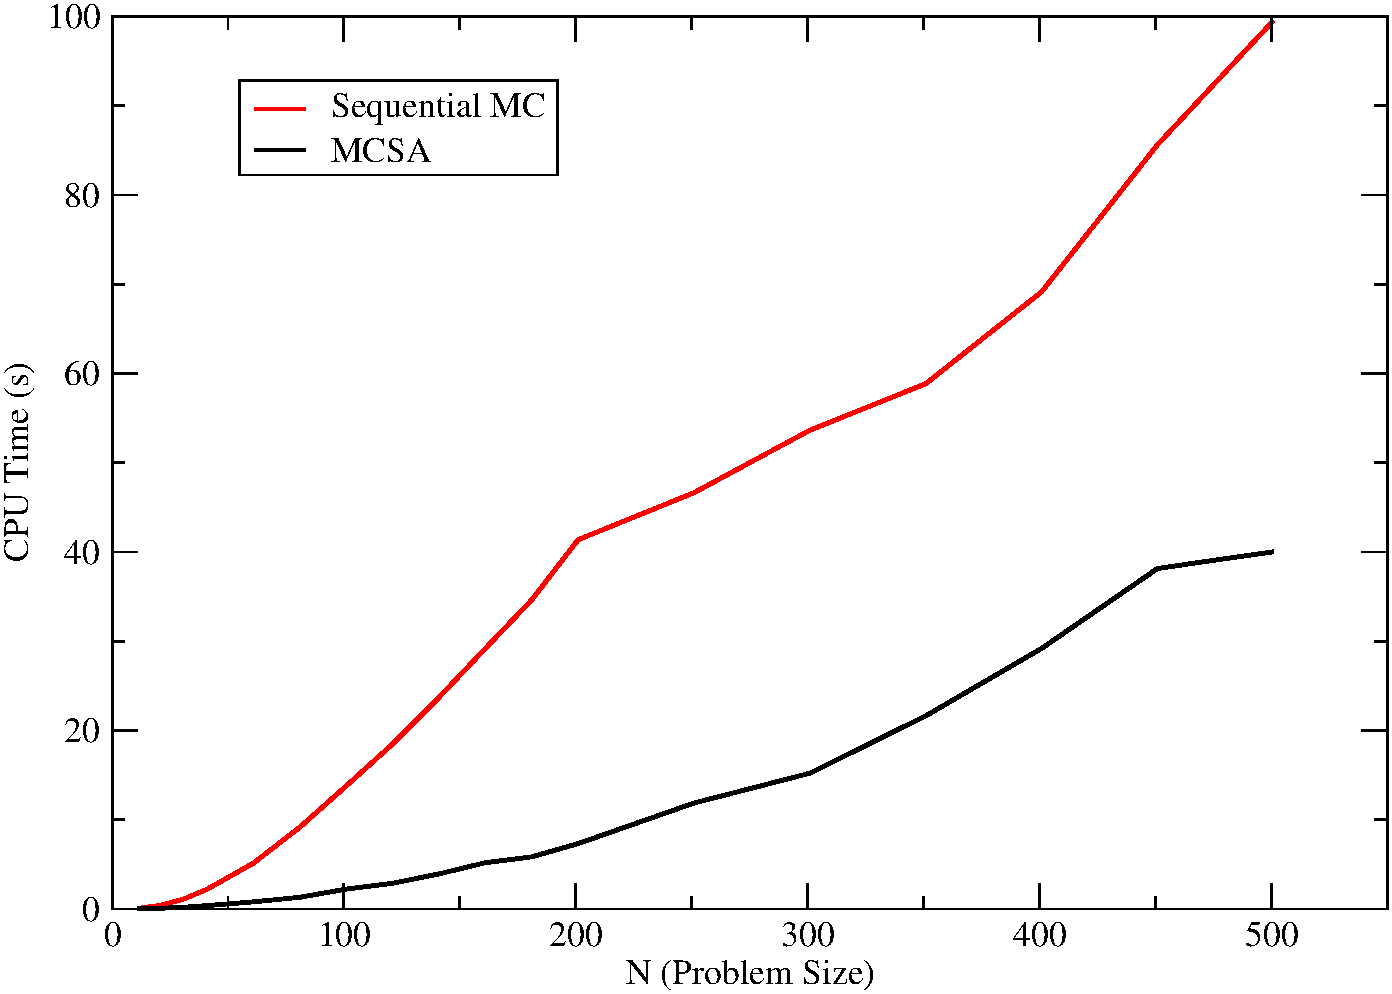
\includegraphics[width=5in,clip]{chapters/mc_background/seq_cpu.pdf}
  \caption{\textbf{CPU Time (s) to converge vs. Problem Size ($N$ for
      an $N \times N$ square mesh).} \textit{oth the Sequential Monte
      Carlo and MCSA solvers are used with the five point stencils and
      the adjoint Monte Carlo solver. The number of random walks was
      twice the number of discrete states in the system in order to
      ensure convergence in the Sequential Monte Carlo method.}}
  \label{fig:seq_cpu_time}
\end{figure}

\begin{figure}[ht!]
  \centering
  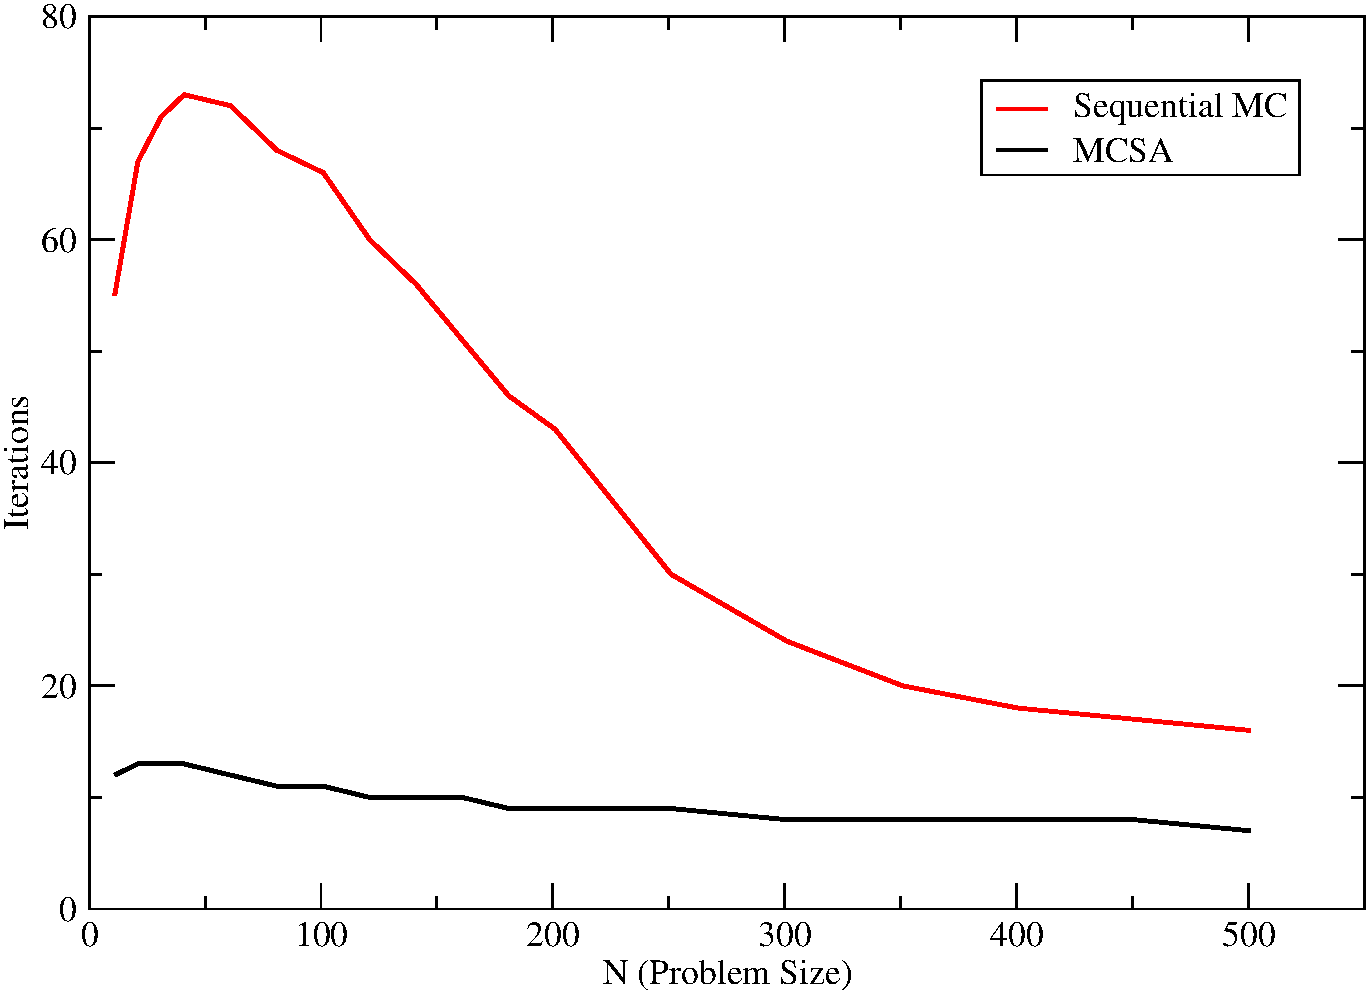
\includegraphics[width=5in,clip]{chapters/mc_background/seq_iterations.pdf}
  \caption{\textbf{Iterations to converge vs. Problem Size ($N$ for an
      $N \times N$ square mesh).} \textit{Both the Sequential Monte
      Carlo and MCSA solvers are used with the five point stencils and
      the adjoint Monte Carlo solver.}}
  \label{fig:seq_iterations}
\end{figure}

The benefits of using a synthetic acceleration scheme are also noted
when the infinity norm of the residual computed at each iteration for
both methods was collected at each iteration for a fixed problem sizes
of $N=100$ and $N=500$ as shown in figures Figure~\ref{fig:seq_100}
and \ref{fig:seq_500} respectively. In both cases, the Sequential
method is subject to two regimes of exponential convergence with the
later regime converging the slowest while the MCSA method exhibits a
single rate of exponential convergence observed to be much higher than
that computed by Halton's method. Even with the doubling of the number
of stochastic histories computed per time step in order to ensure
convergence for the Sequential method, we still see robustness issues
with a non-monotonically decreasing residual observed for the $N=100$
case. In both cases the MCSA solver is observed to be robust with a
monotonically decreasing residual.

\begin{figure}[ht!]
  \centering
  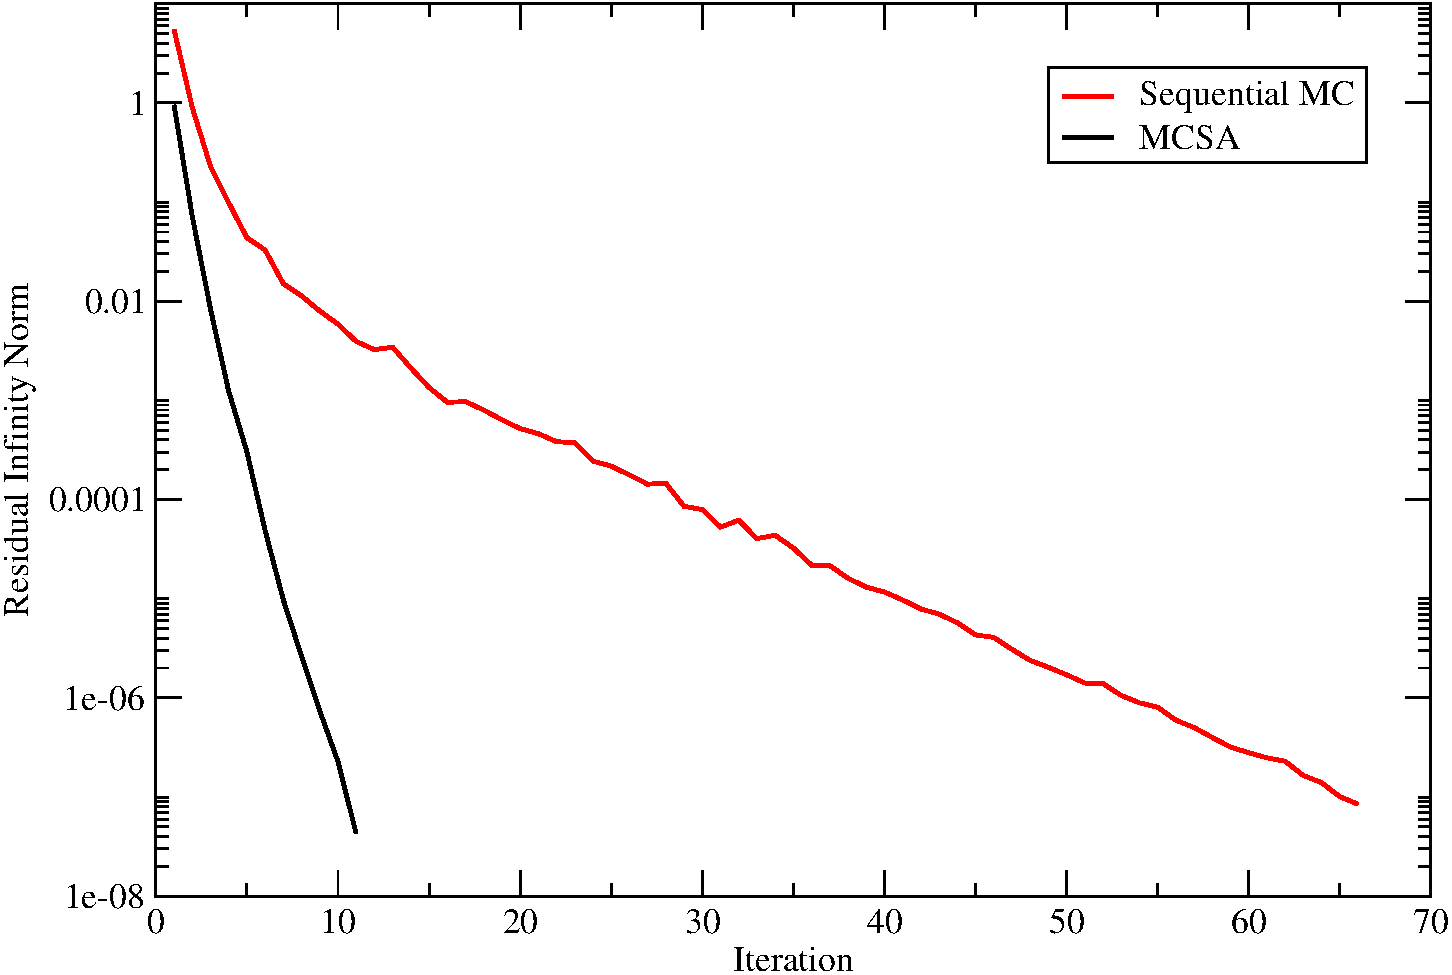
\includegraphics[width=5in,clip]{chapters/mc_background/seq_conv_100.pdf}
  \caption{\textbf{Infinity norm of the solution residual
      vs. iteration number for a problem of size $N=100$.}
    \textit{Both the Sequential Monte Carlo and MCSA solvers are used
      with the five point stencils and the adjoint Monte Carlo
      solver.}}
  \label{fig:seq_100}
\end{figure}

\begin{figure}[ht!]
  \centering
  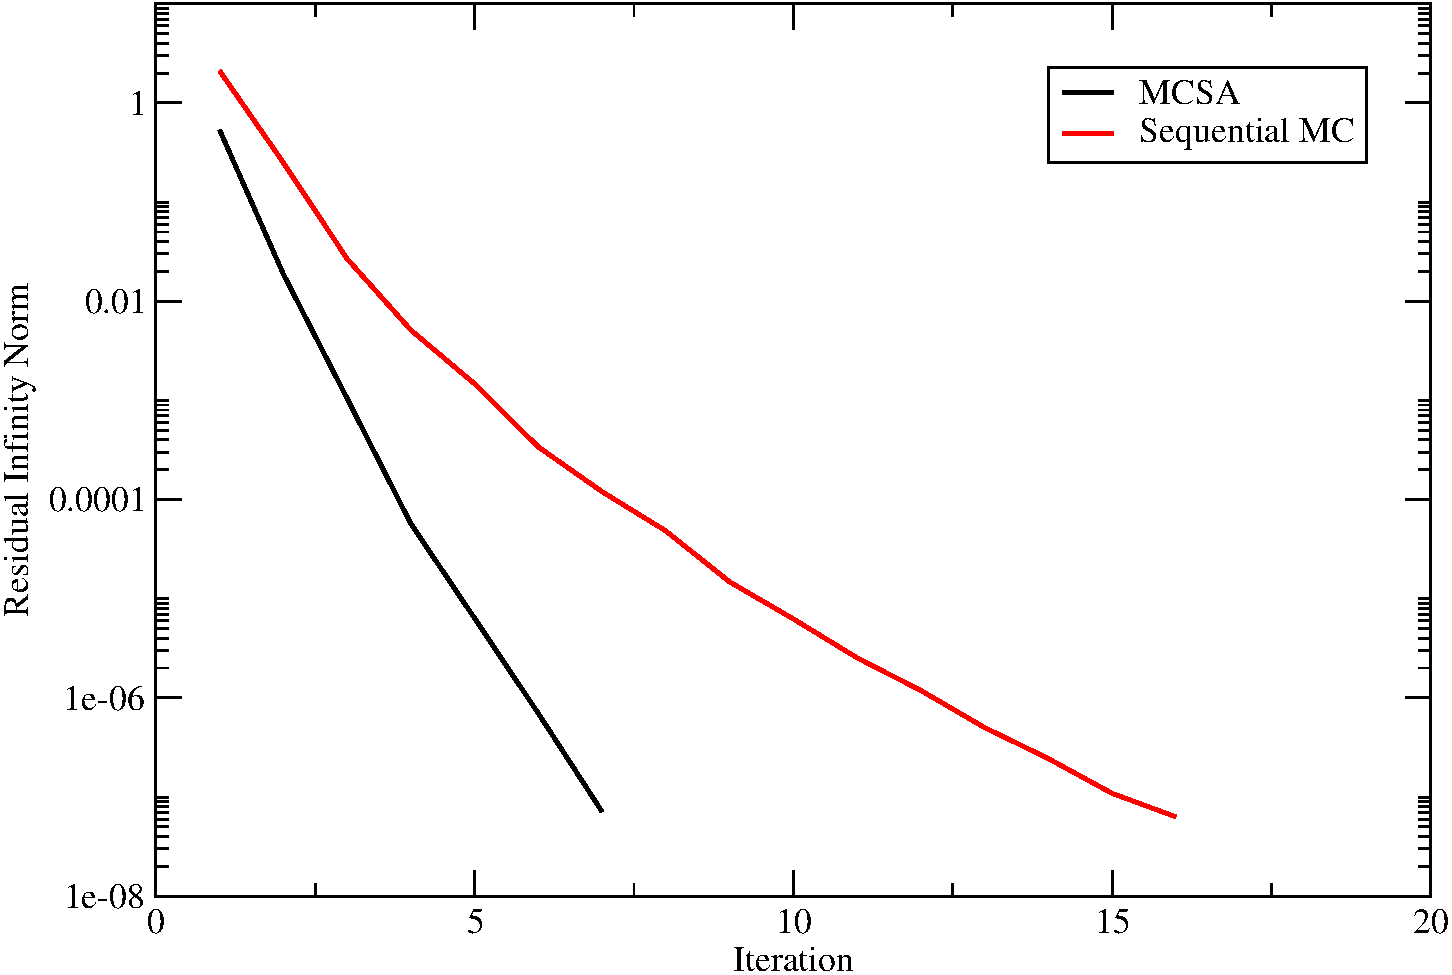
\includegraphics[width=5in,clip]{chapters/mc_background/seq_conv_500.pdf}
  \caption{\textbf{Infinity norm of the solution residual
      vs. iteration number for a problem of size $N=500$.}
    \textit{Both the Sequential Monte Carlo and MCSA solvers are used
      with the five point stencils and the adjoint Monte Carlo
      solver.}}
  \label{fig:seq_500}
\end{figure}

\section{Parallelization of Stochastic Methods}
\label{sec:parallel_stochastic_methods}
For Monte Carlo methods, and in particular MCSA, to be viable at the
production scale, scalable parallel implementations are required. In a
general linear algebra context for discrete systems, this has not yet
been achieved. Therefore, we will develop and implement parallel
algorithms for these methods leveraging both the knowledge gained from
the general parallel implementations of Krylov methods and modern
parallel strategies for Monte Carlo as developed by the reactor
physics community. In order to formulate a parallel MCSA algorithm, we
recognize that the algorithm occurs in two stages, an outer iteration
performing Richardson's iteration and applying the correction, and an
inner Monte Carlo solver that is generating the correction via the
adjoint method. The parallel aspects of both these components must be
considered.

\subsection{Domain Decomposition for Monte Carlo}
\label{subsec:msod}
As observed in the discussion on parallel Krylov methods, large-scale
problems will surely have their data partitioned such that each
parallel process owns a subset of the equations in the linear
system. Given this convention, the adjoint Monte Carlo algorithm must
perform random walks over a domain that is decomposed and must remain
decomposed due to memory limitations. This naturally leads us to seek
parallel algorithms that handle domain decomposition.

In the context of radiation transport, Brunner and colleagues provided
a survey of algorithms for achieving this as implemented in production
implicit Monte Carlo codes \citep{brunner_comparison_2006}. In their
work they identify two data sets that are required to be communicated:
the sharing of particles that are transported from one domain to
another and therefore from one processor to another and a global
communication that signals if particle transport has been completed on
all processors. The algorithms presented are a fully-locking
synchronous scheme, an asynchronous-send/synchronous-receive pattern,
a traditional master/slave scheme, and a modified master/slave scheme
the implements a binary tree pattern for the global reduction type
operations needed to communicate between the master and slave
processes. They observed that the modified master/slave scheme
performed best in that global communications were implemented more
efficiently than those required by the asynchronous
scheme. Furthermore, none of these schemes handled load-imbalanced
cases efficiently. Such cases will be common if the source sampled in
the Monte Carlo random walk is not isotropic and not evenly
distributed throughout the global domain. It was noted that
efficiencies were improved by increasing the frequency by which
particle data was communicated between domain-adjacent
processors. However, this ultimately increases communication costs. In
2009, Brunner extended his work by using a more load-balanced approach
with a fully asynchronous communication pattern
\citep{brunner_efficient_2009}. Although the extended implementation
was more robust and allowed for scaling to larger numbers of
processors, performance issues were still noted with parallel
efficiency improvements needed in both the weak and strong scaling
cases for unbalanced problems. These results led Brunner to conclude
that a combination of domain decomposition and domain replication
could be used to solve some of these issues.

\subsubsection{Multiple-Set Overlapping-Domain Decomposition}
\label{subsubsec:msod}
In 2010, Wagner and colleagues developed the \textit{multiple-set
  overlapping-domain} (MSOD) decomposition for parallel Monte Carlo
applications for full-core light water reactor analysis
\citep{wagner_hybrid_2010}. In their work, an extension of Brunner's,
their scheme employed the similar parallel algorithms for particle
transport but a certain amount of overlap between adjacent domains was
used to decrease the number of particles leaving the local domain. In
addition, Wagner utilized a level of replication of the domain such
that the domain was only decomposed on $O(100)$ processors and if
replicated $O(1,000)$ times achieves simulation on $O(100,000)$
processors, thus providing spatial and particle parallelism. Each
collection of processors that constitutes a representation of the
entire domain is referred to as a set, and within a set overlap occurs
among its sub-domains. The original motivation was to decompose the
domain in a way that it remained in a physical cabinet in a large
distributed machine, thus reducing latency costs during
communication. A multiple set scheme is also motivated by the fact
that communication during particle transport only occurs within a set,
limiting communications during the transport procedure to a group of
$O(100)$ processors, a number that was shown to have excellent
parallel efficiencies in Brunner's work and therefore will scale well
in this algorithm. The overlapping domains within each set also
demonstrated reduced communication costs. On each processor, the
source is sampled in the local domain that would exist if no overlap
was used while tallies can be made over the entire overlapping domain.

To demonstrate this, consider the example adapted from Mervin's work
with Wagner and others in the same area \citep{mervin_variance_2012}
and presented in Figure~\ref{fig:msod_example}.
\begin{figure}[htpb!]
  \begin{center}
    \scalebox{1.5}{
      \input{chapters/mc_background/msod_example.pdftex_t} }
  \end{center}
  \caption{\textbf{Overlapping domain example illustrating how domain
      overlap can reduce communication costs.}
    \textit{All particles start in the blue region of interest. The
      dashed line represents 0.5 domain overlap between domains.}}
  \label{fig:msod_example}
\end{figure}
In this example, 3 particle histories are presented emanating from the
blue region of interest. Starting with particle A, if no domain
overlap is used then the only the blue domain exists on the starting
processor. Particle A is then transported through 3 other domains
before the history ends, therefore requiring three communications to
occur in Brunner's algorithm. If a 0.5 domain overlap is permitted as
shown by the dashed line, then the starting process owns enough of the
domain such that no communications must occur in order to complete the
particle A transport process. Using 0.5 domain overlap also easily
eliminates cases such as the represented by the path of particle C. In
this case, particle C is scattering between two adjacent domains,
incurring a large latency cost for a single particle. Finally, with
particle B we observe that 0.5 domain overlap will still not eliminate
all communications. However, if 1 domain overlap were used, the entire
geometry shown in Figure~\ref{fig:msod_example} would be contained on
the source processor and therefore transport of all 3 particles
without communication would occur.

Wagner and colleagues used this methodology for a 2-dimensional
calculation of a pressurized water reactor core and varied the domain
overlap from 0 to 3 domain overlap (a $7 \times 7$ box in the context
of our example) where a domain constituted a fuel assembly. For the
fully domain decomposed case, they observed that 76.12\% of all source
particles leave the domain. At 1.5 domain overlap, the percentage of
source particles born in the center assembly leaving the processor
domain dropped to 1.05\% and even further for 0.02\% for the 3 domain
overlap. Based on these results, this overlap approach, coupled with
the multiple sets paradigm that will scale for existing parallel
transport algorithms, provides a scalable Monte Carlo algorithm for
today's modern machines.

\subsubsection{Domain-to-Domain Communication}
\label{subsubsec:mc_comm_costs}
With Wagner's work, we observed that domain overlap implemented with a
domain decomposed Monte Carlo setting reduces the amount of nearest
neighbor communication that must occur during transport. This
communication, expected to be expensive, was analyzed by Siegel and
colleagues for idealized, load balanced situations without domain
overlap \citep{siegel_analysis_2012}. They arrive at a few empirical
relationships and generate a numerical experiment that provides
insight into the feasibility of large scale domain decomposed Monte
Carlo as well as the relationship of communication to system
parameters. In their work, they define a simple 3-dimensional system
subdivded into Cartesian block domains with each processor containing
a single domain. Given this geometry, a particle can either be
absorbed in its current domain or be transported to one of the 6
adjacent domains owned by another process.

To quantify the number of particles that leak out of the local domain
they define a leakage fraction, $\lambda$, as:
\begin{equation}
  \lambda =
  \frac{average\ \#\ of\ particles\ leaving\ local\ domain}{total\ 
    of\ \#\ of\ particles\ starting\ in\ local\ domain}\:.
  \label{eq:leakage_fraction}
\end{equation}
For their studies, they assumed that the value of $\lambda$ was
dependent on the total cross section of the system and the same for
all processes for simplicity and load balancing. Using this
relationship and their simple geometry, they were able to relate the
amount of compute time required to transport all source particles to
the number of source particles, the leakage fraction, the latency and
bandwidth of communication, the ratio of local to global geometry
size, and the total cross section of the system.

What they found was that there was indeed an optimum ratio of local
domain to global domain size that results in a minimum total compute
time. They also found that this ratio was only dependent on the
latency and bandwidth constraints of the parallel machine. We expect
this because nearest neighbor communication patterns scale with the
volume and surface sizes of the local domains. The larger the volume,
the more compute time is spent within the local volume and therefore
at some point you are limited by the latency of the system, or the
time it takes to receive the data to operate on. However, at a certain
point, when the surface of those volumes becomes large enough, the
amount of data that must be communicated grows large enough that it
may overcome the bandwidth limitations of the system, resulting in a
decrease in performance. In their numerical experiments, they used the
above geometry and leakage rates based on that computed for a reactor
system for a single material problem with a total cross section
equivalent to that of homogenized light water reactor. Given the
optimal local domain size, they observed for load balanced situations
that nearest neighbor communication costs during transport are a small
fraction of total compute time, leading to the conclusion that domain
decomposition is feasible for large-scale Monte Carlo calculations.

\subsubsection{Load Balancing Concerns}
\label{subsubsec:mc_load_balancing}
Although domain decomposition was shown to be efficient in a perfectly
load balanced situation in Siegel's work \citep{siegel_analysis_2012},
careful consideration must be made for situations where this is not
the case. Given the stochastic nature of the problem and lack of a
globally homogeneous domain, parallel Monte Carlo simulations are
inherently load imbalanced. Procassini and others worked to alleviate
some of the load imbalances that are generated by both particle and
spatial parallelism and are therefore applicable to the MSOD algorithm
\citep{procassini_dynamic_2005}. They chose a dynamic balancing scheme
in which the number of times a particular domain was replicated was
dependent on the amount of work in that domain (i.e. domains with a
high particle flux and therefore more particle histories to compute
require more work). In this variation, domains that require more work
will be replicated more frequently at reduced particle counts in each
replication. Furthermore, Procassini and colleagues noted that as the
simulation progressed and particles were transported throughout the
domain, the amount of replication for each domain would vary as
particle histories began to diffuse, causing some regions to have
higher work loads and some to have smaller work loads than the initial
conditions.

Consider the example in Figure~\ref{fig:procassini_example} adapted
from Procassini's work.
\begin{figure}[htpb!]
  \begin{center}
    \scalebox{1.5}{
      \input{chapters/mc_background/procassini_example.pdftex_t} }
  \end{center}
  \caption{\textbf{Example illustrating how domain decomposition can
      create load balance issues in Monte Carlo.}  \textit{A domain is
      decomposed into 4 zones on 8 processors with a point source in
      the lower left zone. As the particles diffuse from the source in
      the random walk sequence as shown in the top row, their tracks
      populate the entire domain. As given in the bottom row, as the
      global percentage of particles increases in a zone, that zone's
      replication count is increased.}}
  \label{fig:procassini_example}
\end{figure}
In this example, a geometry is decomposed into 4 domains on 8
processors with a point source in the bottom left domain. To begin,
because the point source is concentrated in one domain, that domain is
replicated 5 times such the amount of work it has to do per processor
is roughly balanced with the others. As the particles begin to diffuse
away from the point source, the amount of replication is adjusted to
maintain load balance. Near the end of the simulation, the diffusion
of particles is enough that all domains have equal replication.  By
doing this, load balance is improved as each domain has approximately
equal work although each domain may represent a different spatial
location and have a differing number of histories to
compute. Compared to Wagner's work where the fission source was
distributed relatively evenly throughout the domain, fixed source
problems (and especially those that have a point-like source) like
those presented in Procassini's work will be more prone to changing
load balance requirements.

\subsubsection{Reproducible Domain Decomposed Results}
\label{subsubsec:reproducible_mc}
The 2006 work of Brunner is notable in that the Monte Carlo codes used
to implement and test the algorithms adhered to a strict policy of
generating identical results independent of domain decomposition or
domain replication as derived from the work of Gentile and colleagues
\citep{gentile_obtaining_2005}. In Gentile's work, a procedure is
given for obtaining results reproducible to machine precision for an
arbitrary number of processors and domains. Differences can arise from
using a different random number sequence in each domain and performing
a sequence of floating point operations on identical data in a
different order, leading to variations in round-off error and
ultimately a non-identical answer. They use a simple example,
recreated below in Figure~\ref{fig:gentile_example}, that illustrates
these issues.
\begin{figure}[htpb!]
  \begin{center}
    \scalebox{1.5}{
      \input{chapters/mc_background/gentile_example.pdftex_t} }
  \end{center}
  \caption{\textbf{Gentile's example illustrating how domain
      decomposition can create reproducibility issues in Monte Carlo.}
    \textit{Both particles A and B start in zone 1 on processor
      1. Particle A moves to zone 2 on processor 2 and scatters back
      to zone 1 while B scatters in zone 1 and remains there. A1 and
      A2 denote the track of particle A that is in zone 1 while B1 and
      B2 denote the track of particle B that is in zone 1.}}
  \label{fig:gentile_example}
\end{figure}
In this example, the domain is decomposed on two processors with each
processor owning one of the two zones. Starting with particle A, it is
born in zone 1 and is transported to zone 2 where a scattering event
occurs. Concerning the first reproducibility issue, if the same
sequence of random numbers is not used to compute the trajectory from
the new scattering event, we cannot expect to achieve the same result
if the domain were not decomposed. If the numbers are different, the
scattering event in zone 2 may keep the particle there or even eject
it from the domain if the sequence were different. The second issue is
demonstrated by adding another particle B that remains in the
domain. In this case, an efficient algorithm will transport particle A
on processor 1 until it leaves zone 1 and then transport particle
B. Particle A will not renter the domain until it has been
communicated to processor 2, processor 2 performs the transport, and
it is communicated back to processor 1. If we are doing a track-length
tally in zone 1, then we sum the tracks lengths observed in that
zone. In the single processor, single zone case particle A would be
transported in its entirety and then particle B transported. This
would result in a tally sum with the following order of operations:
$(((A1+A2)+B1)+B2)$. If we were instead to use 2 processors, we would
instead have the following order: $(((A1+B1)+B2)+A2)$. In the context
of floating point operations, we cannot expect these to have an
identical result to machine precision as round-off approximations will
differ resulting in non-commutative addition.

Procassini's solutions to these problems are elegant in that they
require a minimal amount of modification to be applied to the Monte
Carlo algorithm. To solve the first issue, in order to ensure each
particle maintains an invariant random number sequence that determines
its behavior regardless of domain decomposition, each particle is
assigned a random number seed that describes its current state upon
entering the domain of a new processor. These seeds are derived from
the actual geometric location of the particle such that it is
decomposition invariant. Non-commutative floating point operations are
overcome by instead mapping floating point values to 64-bit integer
values for which additions will always be commutative. Once the
operations are complete, these integers are mapped back to floating
point values.

\subsection{Parallel Adjoint Method}
\label{subsec:parallel_adjoint}
We can take much of what was learned from the survey of parallel Monte
Carlo methods for radiation transport and directly apply it to a
parallel formulation of our stochastic linear solvers. Direct analogs
can be derived from these works by noting that the primary difference
between solving a linear system with Monte Carlo methods and fixed
source Monte Carlo transport problems is the content of the Markov
chains that are generated. The transitions represented by these chains
are bound by probabilities and weights and are initiated by the
sampling of a source. In the context of transport problems, those
transitions represent events such as particle scattering and
absorption with probabilities that are determined by physical data in
the form of cross sections. For stochastic matrix inversion, those
transitions represent moving between the equations of the linear
system (and therefore the physical domain which they represent) and
their probabilities are defined by the coefficients of those
equations. Ultimately, we tally the contributions to generate
expectation values in the desired states as we progress through the
chains. Therefore, parallel methods for Monte Carlo radiation
transport can be abstracted and we can use those concepts that apply
to matrix inversion methods as an initial means of developing a
parallel Neumann-Ulam-type solver. Based on the results observed in
the last decade of parallel Monte Carlo development, we can generate
many practical questions that this type of work could answer.

Given a decomposed domain, per Wagner's work
\citep{wagner_hybrid_2010} is clear that domain overlap significantly
reduces the amount of communication required between adjacent domains
as histories move to states that are not owned by the local
processor. How much domain overlap is suitable for matrix inversion
problems? Are we memory limited by large problems such that only so
much overlap is feasible? Are there metrics related to the properties
of the matrix including the eigenvalues and sparsity pattern such that
we can provide guidelines for selecting the amount of overlap
required? Furthermore, as Wagner and colleagues observed
\citep{wagner_hybrid_2010}, with marginal domain overlap for reactor
problems, the percentage of histories leaving the local domain can
easily be reduced to less than 1\%. Evans and colleagues in their
initial MCSA development typically used only 50 particle histories in
order to compute a correction in an MCSA iteration
\citep{evans_monte_2012}. Per the Central Limit Theorem, that
correlates to a statistical uncertainty of 14.1\% in the correction,
yet as compared to conventional Krylov solvers, MCSA achieved
identical numerical results. If good convergence and numerically
accurate solutions can be achieved with such a large uncertainty in
the correction computation, then perhaps with enough domain overlap
the minimal amount of histories that do transition to non-local states
can be ignored and thus eliminate all communication in the parallel
Monte Carlo adjoint solver transport sequence and create an
embarrassingly parallel method. Given Gropp's work on parallel Krylov
methods that we discussed in
\S~\ref{subsec:projection_method_performance} and the empirical
results of Siegel \citep{siegel_analysis_2012}, we know that these
nearest neighbor computations between adjacent domains do not scale as
well as global reduction operations and therefore we are improving
scaling by eliminating them from the transport sequence. It will be
important to determine if the expectation value bias in the MCSA
correction generated by this approximation will remain within the
bounds of the already high statistical uncertainty for unbiased
estimates, thus providing numerically equivalent results.

From a domain replication perspective, this may be difficult to
achieve with a production scale linear solver. Typically, memory is at
a premium and therefore the more distinct domains available in the
decomposition, the spatially finer and/or the numerically more
accurate the discretization that can be implemented. How much
replication is possible for large problems? How does replication
facilitate parallel performance when coupled with domain overlap? How
can we measure how much domain overlap is feasible? Replicating
domains may therefore run into memory limitations for exceptionally
large problems such that the operator, solution vector, and source
vector must be copied in their entirety multiple times. From a
resiliency standpoint, such an operation will be required, and
therefore its performance and memory implications on conventional
problems must be analyzed.

\subsection{Parallel MCSA}
\label{subsec:parallel_mcsa}
With a parallel adjoint Neumann-Ulam solver implementation, the
parallel implementation of the MCSA method will be trivial. Recall the
MCSA iteration procedure outlined in Eq~(\ref{eq:mcsa}). In
\S~\ref{sec:parallel_krylov_methods} we discussed parallel matrix and
vector operations as utilized in conventional Krylov methods. We
utilize these here for the parallel MCSA implementation. In the first
step, a parallel matrix-vector multiply is used to apply the split
operator to the previous iterate's solution. A parallel vector update
is then performed with the source vector to arrive at the initial
iteration guess. In the next step, the residual is computed by the
same operations where now the operator is applied to the solution
guess with a parallel matrix-vector multiply and then a parallel
vector update with the source vector is performed. Once the correction
is computed with a parallel adjoint Neumann-Ulam solve, this
correction is applied to the guess with a parallel vector update to
get the new iteration solution. Additionally, as given by
Eq~(\ref{eq:mcsa_stopping_criteria}), 2 parallel vector reductions
will be required to check the stopping criteria: one initially to
compute the infinity norm of the source vector, and another at every
iteration to compute the infinity norm of the residual vector. For
this implementation, all of the issues that will be potentially
generated by the parallel adjoint solver implementation will manifest
themselves here as the quality of the correction will be of intense
study.

In addition to parallel implementation and performance, MCSA's
potential for aiding advancement in non-symmetric matrix solutions
leads to a natural comparison with the GMRES algorithm. As both
solvers are aimed at the same class of problem, we desire a set of
metrics that will allow us to quantitatively compare the two. Given
that the Krylov subspace maintained by GMRES can become large, do we
benefit from a memory standpoint with an MCSA scheme in that no
subspace is required? Does this benefit outweigh the fact that the
linear operator must be explicitly formed in order to build the
transition probabilities for the random walk sequence? For
non-symmetric systems, does MCSA exhibit similar convergence
properties to Krylov methods? If a Krylov methods build a subspace,
can those memory savings in MCSA be used to implement domain
replication in the adjoint solver? Such questions can be answered by a
comparative study of the two solvers that controls the system size and
the iterations required to converge.
